% Figures for Pi, Screen and Power Consumption
\begin{figure*}[t]
  \begin{minipage}[t]{0.22\textwidth}
    \centering
    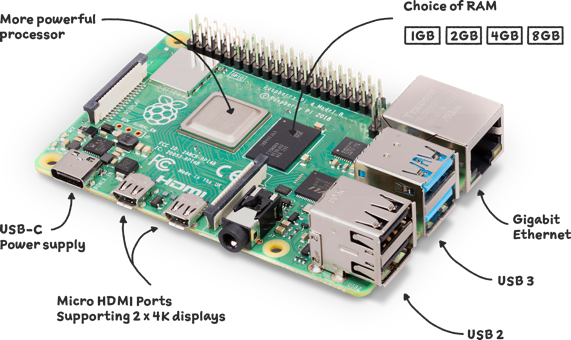
\includegraphics[width=\textwidth,height=5cm, keepaspectratio]{imgs/parts/pi4_labelled.png}
    \caption{Raspberry Pi 4 Model B 2GB \cite{pi4}}
  \end{minipage}
  \hfill
  \begin{minipage}[t]{0.22\textwidth}
    \centering
    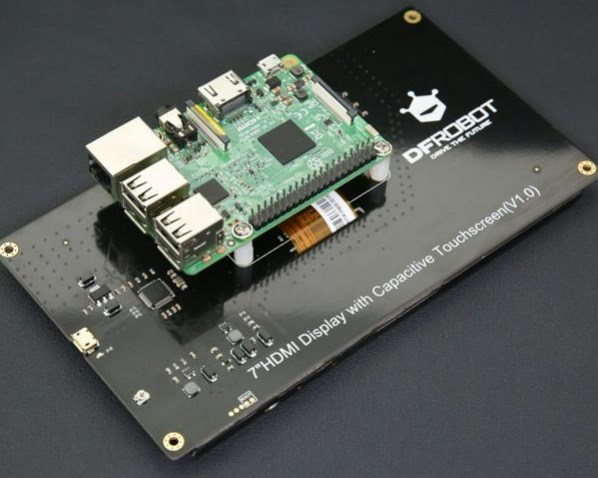
\includegraphics[width=\textwidth,height=5cm, keepaspectratio]{imgs/parts/dfrobot_screen.jpg}
    \caption{DFRobot 7" Touchscreen Display \cite{7inchdisplay}}
  \end{minipage}
  \hfill
  \begin{minipage}[t]{0.22\textwidth}
    \centering
    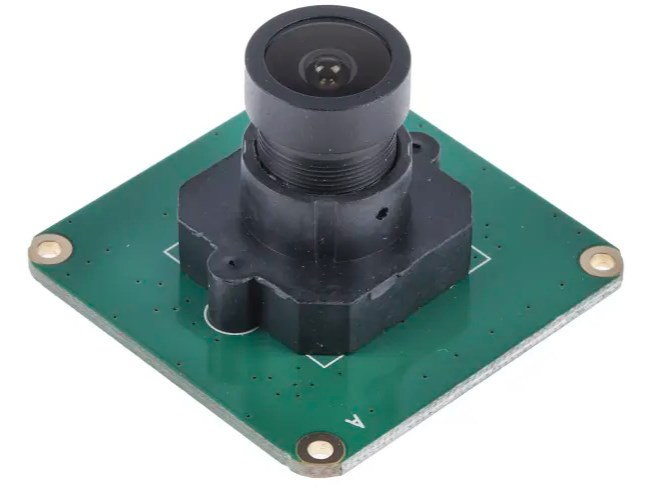
\includegraphics[width=\textwidth,height=5cm, keepaspectratio]{imgs/parts/okdo_camera.jpg}
    \caption{Okdo Adjustable Focus OV5647 Camera \cite{okdocamera}}
  \end{minipage}
  \hfill
  \begin{minipage}[t]{0.22\textwidth}
      \centering
      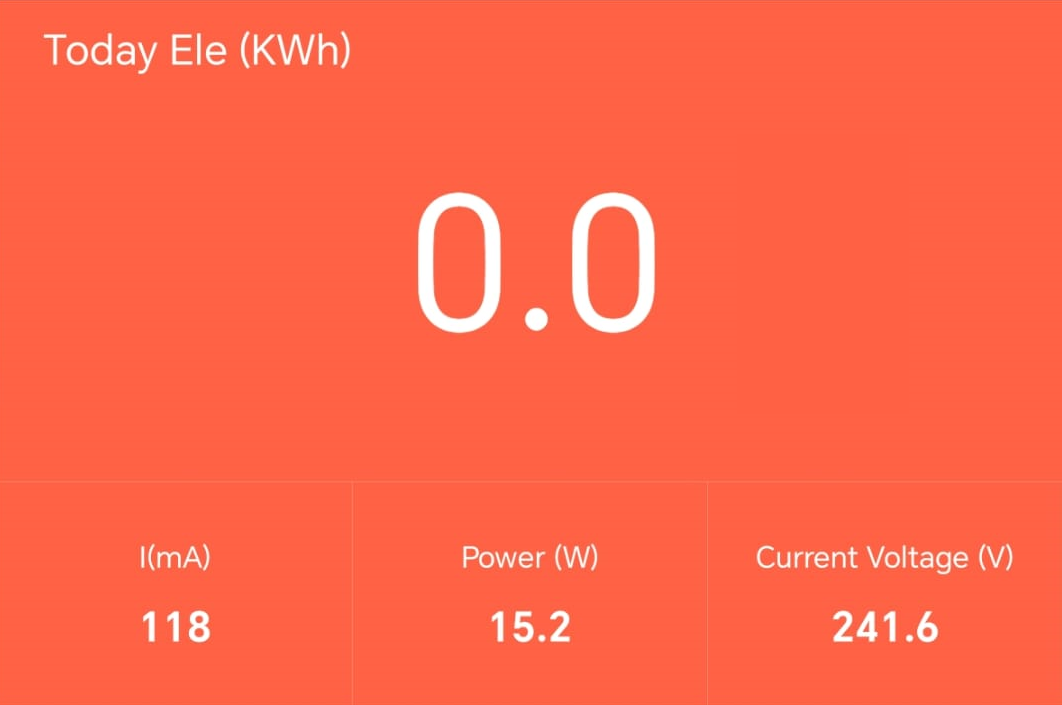
\includegraphics[width=\textwidth,height=5cm, keepaspectratio]{imgs/parts/powermeter.png}
      \caption{Power consumption of the system}
      \label{fig:powermeter}
  \end{minipage}
\end{figure*}

\subsection{Hardware, Mechanics \& Electronics}
The hardware, mechanics and electronics (HME) of the system are the physical components that make up the system.
It is necessary to first consider the HME of the system as they are the foundation upon which the rest of the system is built upon;
for example, when designing the computer vision system, it should utilise training data that was collected using the HME 
that the system will be deployed on, ensuring that the system is robust to the conditions it will be used in.

To keep track of the HME, a spreadsheet was created that contains all the components of the system (otherwise known as the Bill of Materials or BOM),
as well as the cost of each component. A sample of this spreadsheet can be found in Appendix Figure \ref{app:bom}.
\subsubsection{Hardware} \label{sec:hardware}
The following hardware components have been used in the system:
\begin{mylist}
  \item Raspberry Pi 4 Model B 2GB \cite{pi4}
  \item 7" Touchscreen Display \cite{7inchdisplay}
  \item 24V dc, 6.25A, 150W Power Supply
  \item Okdo Adjustable Focus OV5647 Camera \cite{okdocamera}
  \item LED Light Ring
  \item NEMA17 42-40 Stepper Motor + DRV8825 Driver
\end{mylist}
% Pi
\textbf{Raspberry Pi 4 Model B 2GB} \\
The Raspberry Pi 4 Model B was chosen as the main component of the system and is the central hub that all other components are connected to.
This model was chosen as it is regarded as a reliable SoC (System on Chip), is widely used in the industry and was used in the module ELEC96018 Embedded Systems.
It has a large amount of software and driver support, ensuring confidence in finding solutions to any potential issues that may arise. Additionally, 
it has GPIO pins that can be used to control other components. It also has a 
dedicated CSI camera port which allows for a camera to be connected directly to the SoC, which is necessary for the computer vision system.

It also has WiFi support, allowing for SSH and remote development software, as well as an HDMI port for the display.
Originally, the 4GB model was ordered however an issue with the EE Stores resulted in receiving the 2GB model instead.
This was not an issue as the 2GB model was sufficient for the project. The decision to not return the 2GB model is because it was not 
possible to order a new Pi without returning the old one, halting the development of the system.

An alternative to the Pi family of SoCs are Arduinos, but while they are capable of controlling the components of the system,
and potentially drive an LCD, the microcontrollers are typically not powerful enough to run the computer vision system and stream video from the camera,
so they cannot be used as a replacement for the Pi.

A viable alternative to the Pi is a NVIDIA Jetson Nano \cite{jetsonnano}, as it is designed for computer vision applications and has a dedicated GPU. The dedicated GPU
would reduce the likelihood of the computer vision system being a bottleneck, and it has a CSI port for the camera; in terms of CPU performance, the Nano is weaker than the Pi,
having a quad-core ARM Cortex-A57, whereas the Pi has a quad-core ARM Cortex-A72 \cite{pi4}. However, the worse CPU performance is offset by the dedicated GPU, and the Nano has 4GB of RAM, 
making the Nano a very attractive alternative to the Pi. The Nano's drawback is that it is significantly more expensive than the Pi (up to 3x from retailers), and
given the ability to optimise the computer vision system as discussed in Section \ref{sec:background} (Background), the Pi is still
a viable choice for the computer vision system.

To address the lack of a dedicated GPU for inference, an article from Medium \cite{benchmarks} benchmarked the Pi's performance on various computer vision tasks with 
various accelerators like the Intel Neural Compute Stick 2 and the Google Coral USB Accelerator against other SoCs like the Jetson Nano and the Coral Dev Board. 
It was found that the Coral Dev Board was the best performing, however the Pi using optimisation libraries like TensorFlow Lite showed  promising results, which
helps to strengthen the argument for using the Pi for the computer vision system, especially with the SparseML and DeepSparse libraries that were discussed in Section \ref{sec:background} (Background).

The benchmarks can be found in Appendix Figure \ref{app:benchmarking}.

% Screen
\vspace{1em}
\noindent
\textbf{7" Touchscreen Display} \\
The DFRobot 7" Touchscreen Display was chosen as it is a relatively cost-effective display that is compatible with the Raspberry Pi.
It has touchscreen support and has a Raspberry Pi 4 mount on its back, as well as HDMI adapter boards to connect to the Pi.
This means that a physical mount for the Pi does not need to be designed, and only a mount for the display is required. The display is also powered by the Pi,
so no additional power supply is required. 

% Power Supply
\vspace{1em}
\noindent
\textbf{24V dc, 6.25A, 150W Power Supply} \\
Two parameters were taken into consideration when choosing a power supply: the power output and the voltage.
\begin{mylist}
  \item \textbf{Power Rating} \\
  The power supply must be able to drive all components in the system with overhead in case of spikes in power consumption.
  In this first stage, the system only consists of the Raspberry Pi, the display, LED lights and the camera, 
  making for a power consumption of under 20W, recorded using a smart plug with a power meter as shown in Figure \ref{fig:powermeter}.
  However, in the future, the system will likely need to drive additional motors and sensors, so the total power consumption
  will be higher. Even with accounting for this, the power consumption will be under 100W, so a 150W power supply will be sufficient,
  allowing a 50W overhead. In hindsight, this may be considered excessive.
  \item \textbf{Voltage Rating} \\
  The voltage of the power supply must be greater than or equal to the highest voltage of any component in the system; this is necessary
  as there are only step-down converters available on hand, so choosing a higher voltage allows the stepping down of the higher voltage 
  to the required voltage for each component. 24V was chosen as it is a common voltage for stepper motors, which may be used in
  future stages of the project. It is also used for some LED strips, which are used in this stage. The Pi 4 uses 5V and the LED Ring
  uses 12V, which the 24V power supply can be stepped down to.
\end{mylist}

% LED 
\noindent
\textbf{Okdo Adjustable Focus OV5647 Camera} \\
For the Computer Vision system, a camera is required to capture images of the components. The Okdo Adjustable Focus OV5647 Camera
was chosen as it is CSI compatible, meaning it can be connected directly to the Raspberry Pi, and has a manual focus ring, allowing
it to be used as a macro camera to capture images of small components placed directly above it. The manual focus ring allows the camera
to be specifically tuned to the design of the system, allowing for the best possible image quality. It also
has a 5MP sensor \cite{okdospec}, which is sufficient for the computer vision system, as high-resolution images would be preprocessed and reduced,
only adding to the amount of processing required.

% LED
\vspace{1em}
\noindent
\textbf{LED Light Ring} \\
An LED Ring is required to illuminate the components so that the camera can capture images of them.
Initially, a 12V LED Ring was chosen as it would allow for a uniform light source and could be mounted directly below the camera; 
however, for reasons explained in the next section, it was replaced with a 5V WS2812B LED strip as it solves the issues
faced with the LED Ring.
